% \documentclass[master]{styles/hdu-thesis}
\documentclass[master,draft]{styles/hdu-thesis}
%%%%%%%%%%%%%%%%%%%%%%%%%%%%%%%%%%%%%%%%%%%%%%%%%%%%%%%%%%%%%%%%%%%%
%%\documentclass[master]{hdu-thesis}[]中不同的模式选择对应不同的模板%%%%
%|bachelor_p| 本科生毕业论文模板 |
%|bachelor_d| 本科生毕业设计模板 |
%|bachelor_review| 本科生送审模板 |
%|master| 学术型硕士模板 |
%|promaster| 专业学位硕士模板 |
%|doctor| 博士学位模板 |
%|engdoctor| 工程博士学位模板 |
%|master_review| 学术型硕士送审模板 |
%|promaster_review| 专业学位硕士送审模板 |
%|doctor_review|  学术型博士送审模板 |
%|engdoctor_review|  工程博士送审模板 |

%%%%%%%%%%%%%%%%%%%%%%%%%%%%%%%%%%%%%%%%%%%%%%%%%%%%%%%%%%%%%%%%%%%%%%


\title{杭州电子科技大学Latex毕业论文模板使用方法}{Munual of latex on thesis for HDU}
\author{张三}{San Zhang}%%%%%%作者
\advisor{王老师}{Teacher Wang}%%%%%%指导老师
\school{自动化学院}{School of Automation}%%%%学院
\major{控制理论与控制工程}{Control Science and Engineering}%%%%%%%%%%专业
\authornumber{20212021}{} %%%%%%学号
\authorclass{171819} %%%%%%%%%班级(本科生填)
\completedate{2021}{12}{Dec}  %%%%%%设计完成时间
\authordirection{自主移动机器人}{AGV}%%%%研究方向前者对应中文方向,后者对应英文(研究生写)

\begin{document}

%%%%%%%%%%%%%%%%插入封面%%%%%%%%%%%
\makecover
%%%%%%%%%%%%%%%%插入原创性声明%%%%%%%%%
\makedeclaration

%%%%%%%%%%%%%%%中文摘要%%%%%%%%%%%%%%
	
\cnabstract


我不去想,是否能够成功,既然选择了远方,便只顾风雨兼程。

我不去想,能否赢得爱情,既然钟情于玫瑰,就勇敢地吐露真诚。

我不去想,身后会不会袭来寒风冷雨,既然目标是地平线,留给世界的只能是背影。

我不去想,未来是平坦还是泥泞,只要热爱生命,一切,都在意料之中。




\cnkeyword{Latex,热爱生命,汪国真}


%%%%%%%%%%%%%%%英文摘要%%%%%%%%%%%%
\enabstract

I don't want to think about whether I can succeed. Since I have chosen the distance, I only care about the wind and rain.

\enkeyword{Latex, thesis}




% 草稿加入 TODO list
\ifdraft{
  \listoftodos
}{}
% 图目录
\figurelist

% 表格目录
\tablelist

% 缩略词列表
\inputAndPrintGlossaries

% 目录
\tableofcontents

\chapter{绪论}
  绪论一般包含三部分内容:研究背景及意义、国内外研究现状、研究内容三部分。
  \section{研究背景及意义}
  \section{国内外研究现状}
  \section{研究内容}

\ifdraft{
  \chapter{大论文撰写技巧}

\section{参考文献说明}
\subsection{文中参考文献的插入说明}
参考文献有两种格式引入\verb+\cite{}+以及\verb+\citep{}+。使用效果可见下面介绍:\\
1.插入会议inproceedings\upcite{zhao2015bearing0}\\
2.插入教材课本book\upcite{williams1991probability,chengzhaolin2006,zhangsan2007}\\
3.插入期刊article\upcite{cao2011formation,xue2015formation}\\
4.插入硕博论文thesis\upcite{lisi2015,wangwu2015,deans2005bearings}\\
5.插入网站misc\upcite{irdawebsite,h7n9,wikipedia_moores_law}\\
6.插入专利patent\upcite{xiao2012yi,p6915001}\\
7.插入新闻news报纸newspaper\upcite{zhang2000,renminribao}\\
8.插入标准standard\upcite{gbt3469-1983}

\textcolor{red}{注意1:参考文献格式不正确可能导致编译不通过,大家可以参考本工程中reference.bib中文献格式对网上下载不规范的bibtex文件进行修改。此外,如果上述类型里面条目有缺失会会导致编译不能输出正确格式。}

关于参考文献不同类型的进一步详细的说明可参考网站\url{https://github.com/Haixing-Hu/GBT7714-2005-BibTeX-Style}
里面的测试模板。


\textcolor{red}{注意2:对于中文参考文献,为了保证格式正确,最好需在对应bib里面添加\text{language=\{zh\}},不加会默认当做英文文献处理。区别如图\ref{fig_bib0}。}

\begin{figure}[!htb]
  \centering
  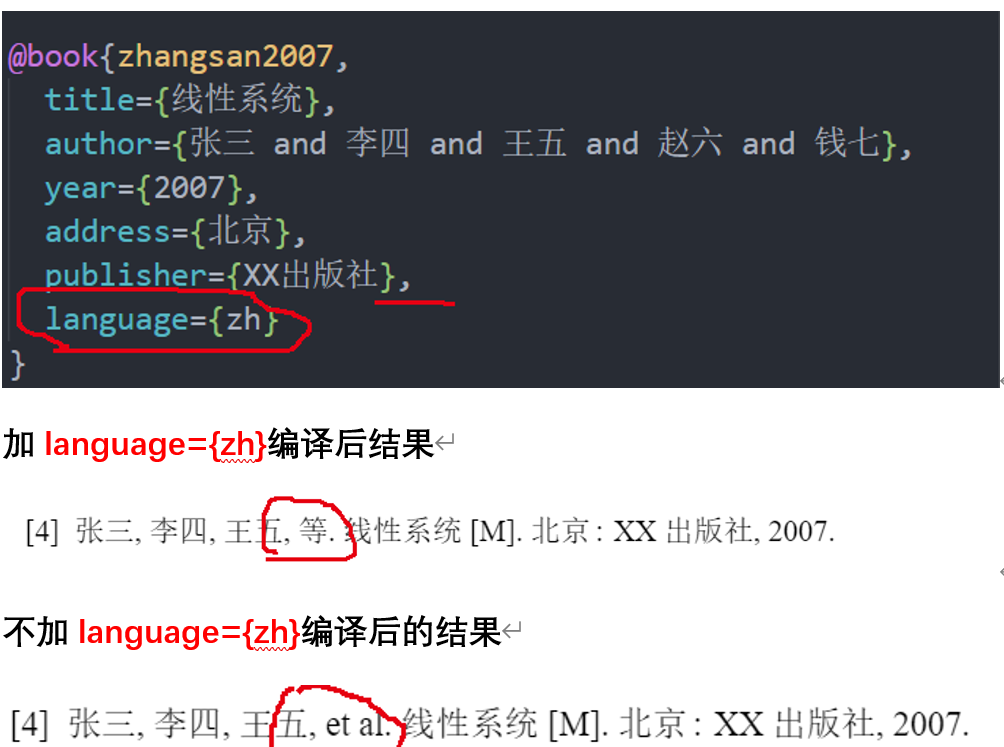
\includegraphics[width=1\textwidth]{manual/figures/中英文文献bib编译注意事项}
  \caption{中英文文献bib编译注意事项以作者超过3个为例进行说明}
  \label{fig_bib0}
\end{figure}

\subsection{参考文献的查找与引用}


多智能体系统\citep{cao2011formation}。
可以通过百度学术搜索查找参考文献(如图\ref{fig_search0}),
 \begin{figure}[!htb]
  \centering
  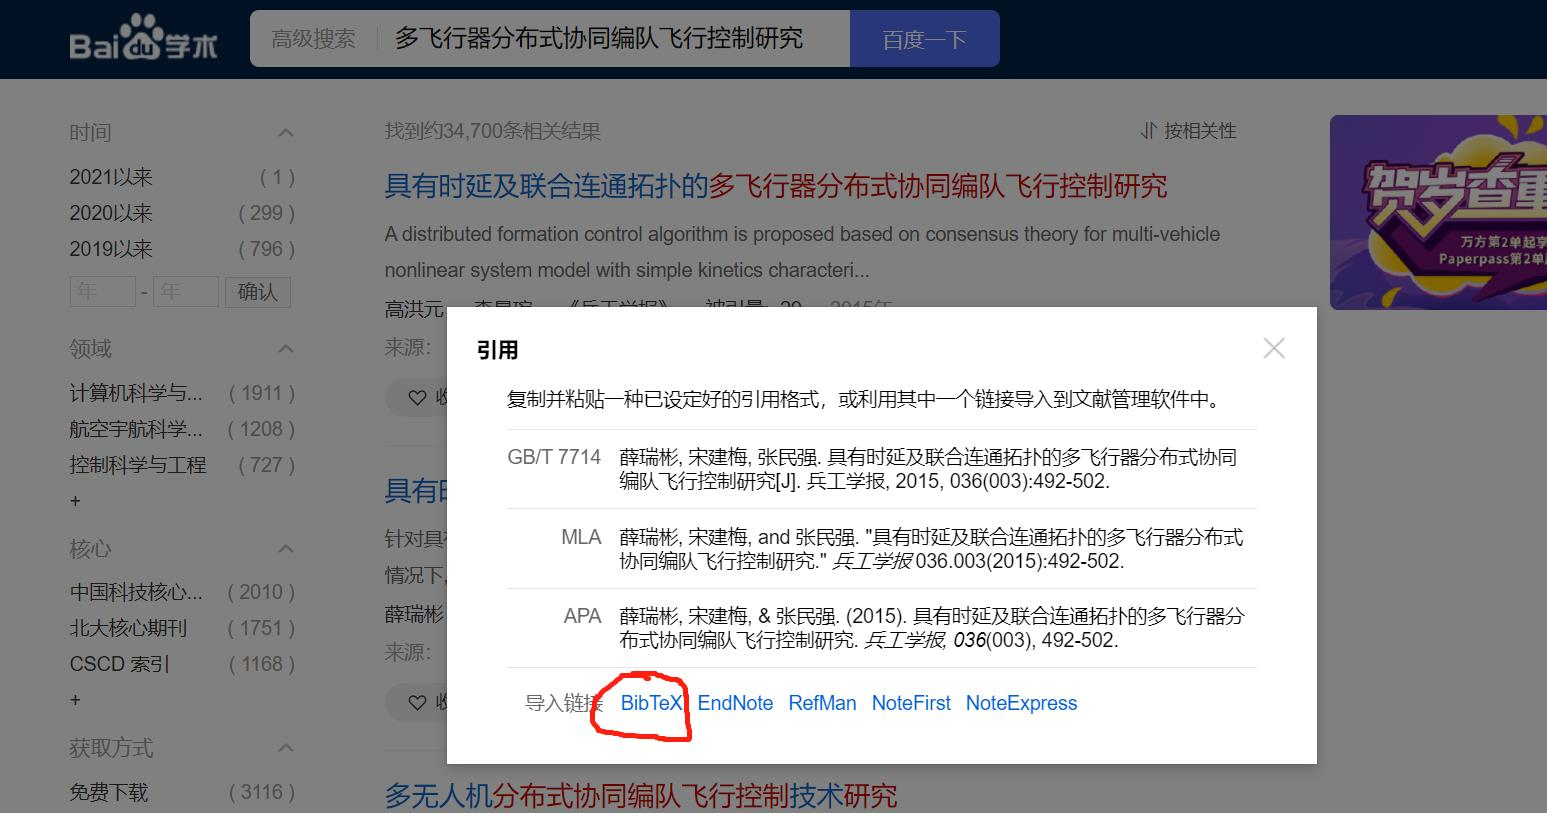
\includegraphics[width=1\textwidth]{manual/figures/文献搜索说明0}
  \caption{参考文献的百度学术搜索.}
  \label{fig_search0}
\end{figure}
点击bibtex,然后复制到目录文件夹中的bib文件(如图\ref{fig_search1})。此时可以调用指令为\citep{薛瑞彬2015具有时延及联合连通拓扑的多飞行器分布式协同编队飞行控制研究}。但是此时标签太长,可以适当修改标签再引用,例如把bib中的标签(第一行)的``薛瑞彬2015具有时延及联合连通拓扑的多飞行器分布式协同编队飞行控制研究"改成``xue2015formation",指令为\verb+\cite{xue2015formation}+,效果为\cite{xue2015formation}。如果进一步想管理参考文献,可新建几个bib文件并用\verb+\bibliography{en_ref,cn_ref,...}+完成。
 \begin{figure}[!htb]
  \centering
  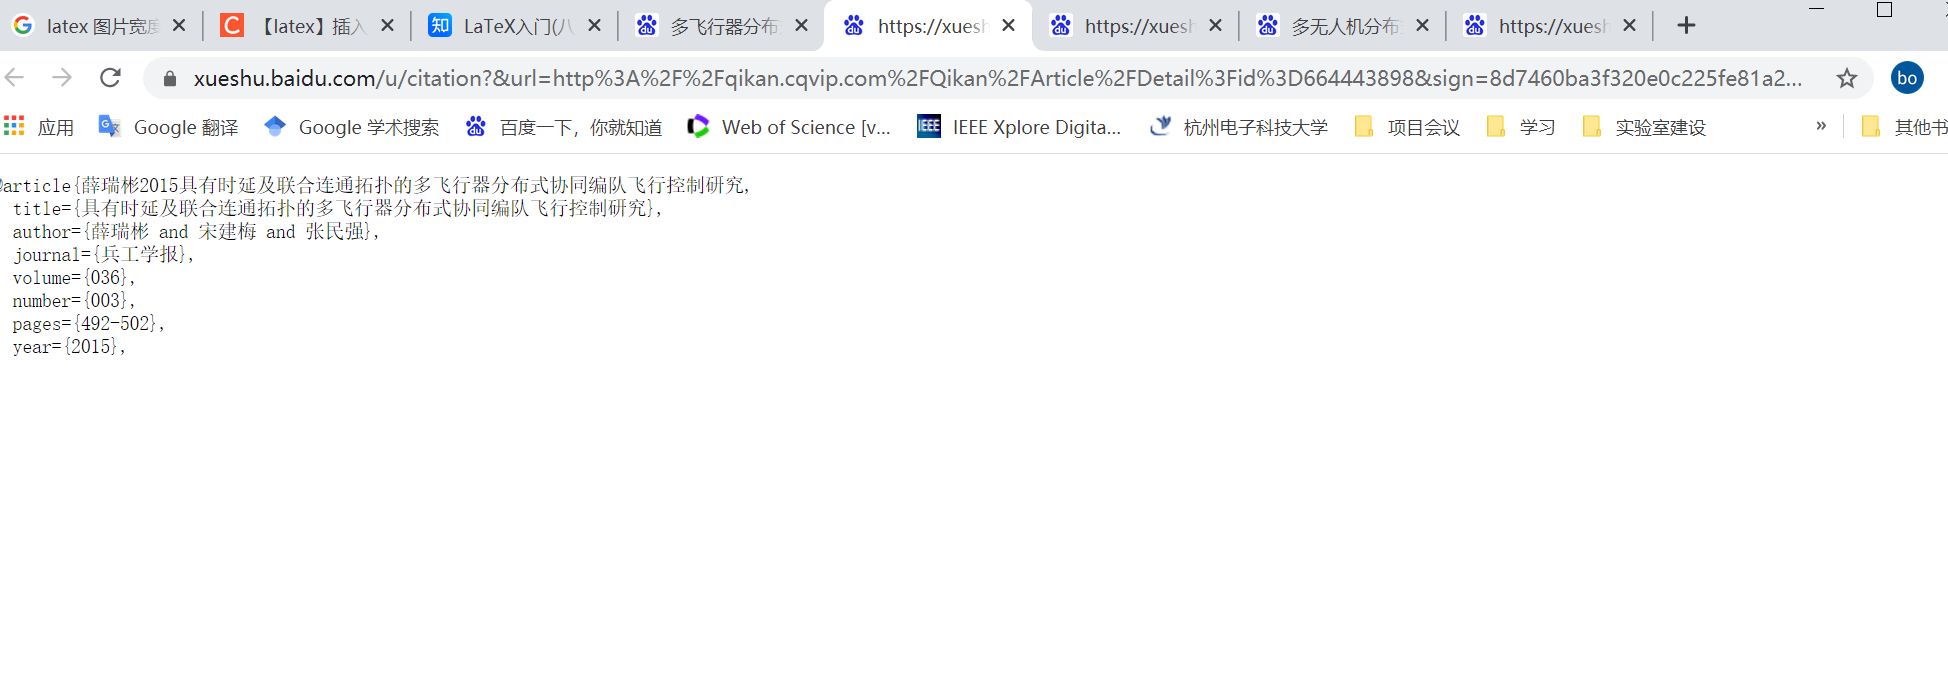
\includegraphics[width=1\textwidth]{manual/figures/文献搜索说明1}
  \caption{参考文献复制到bib文件.}
  \label{fig_search1}
\end{figure}



\section{插入项目符号}

多智能体系统在多方面多领域得到了广泛的应用:
\begin{itemize}
  \item 军事
  \item 政治
  \item 历史
\end{itemize}

\subsection{插入项目编号}

\begin{enumerate}[leftmargin=2em,itemsep=2pt,topsep=0pt,parsep=0pt,label=\alph*)]
  \item 开发目标;
  \item 融合图像。
\end{enumerate}

enumerate不同编号\verb+\Alph*,\alph*,\Roman*,\roman*,\arabic*+
系统的分类:

多智能体系统的分类:
\begin{enumerate}
  \item 同构多智能体系统
  \item 异构多智能体系统
\end{enumerate}

\section{公式的对齐与引用}

\subsection{安装mathtype}
安装mathtype并根据下图完成配置(图\ref{fig_mathtype1}所示)。
 \begin{figure}[!htb]
  \centering
  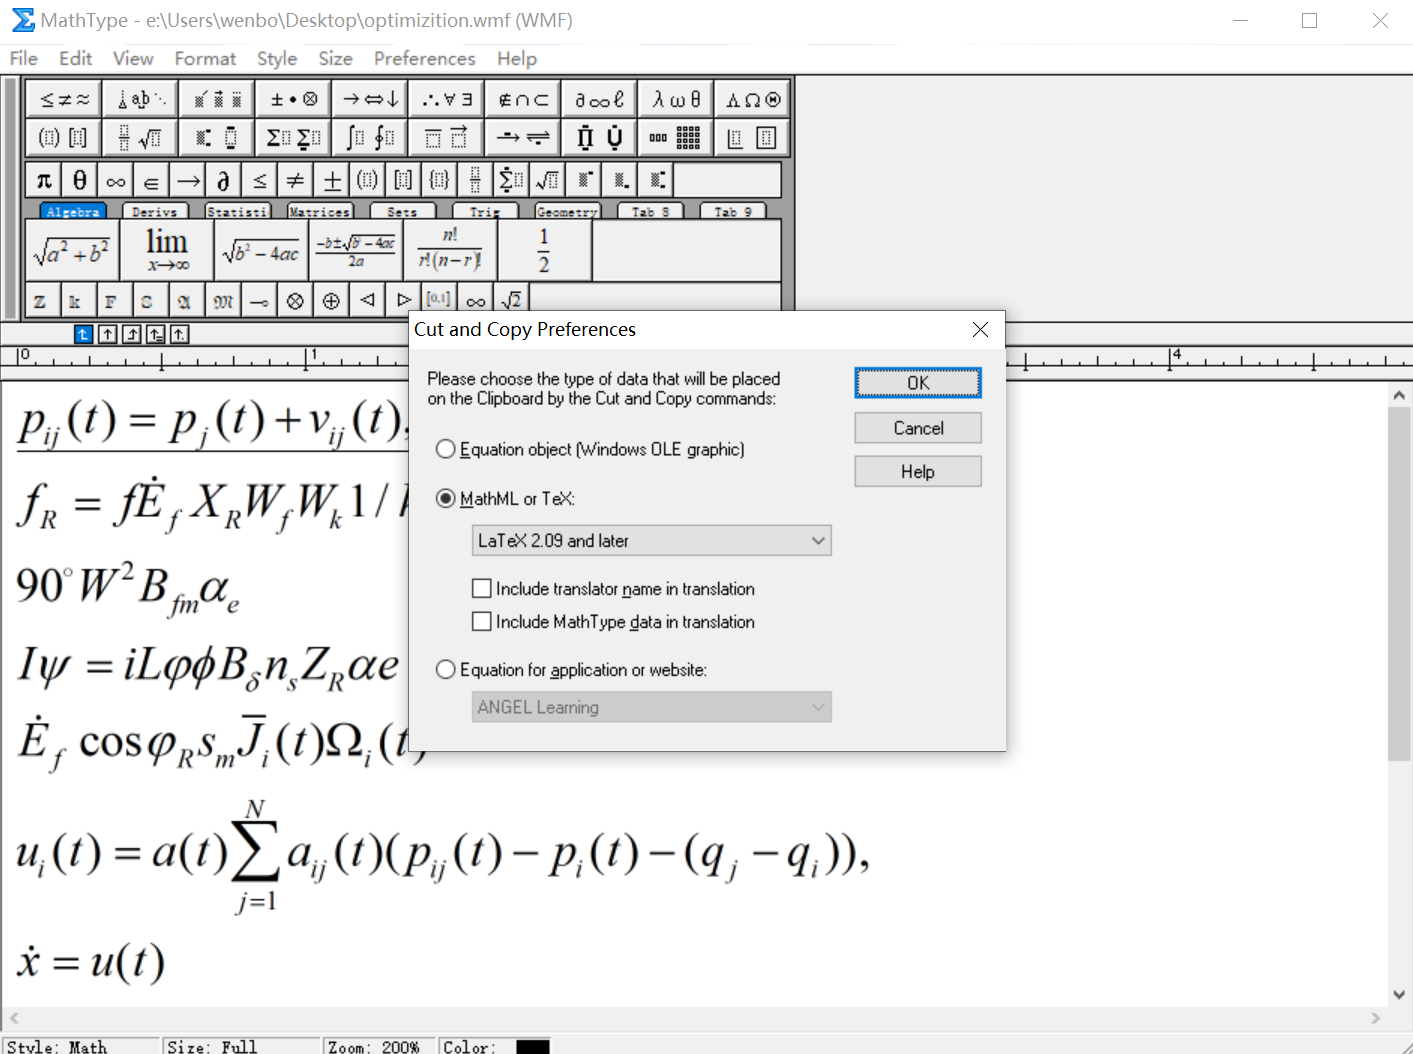
\includegraphics[width=1\textwidth]{manual/figures/mathtype配置}
  \caption{mathtype相关配置.}
  \label{fig_mathtype1}
\end{figure}

\subsection{插入带编号的公式及不带编号的公式}
在mathtype编辑公式,并从mathtype直接复制到latex,然后进一步修改。

\textcolor{red}{在文字段落中嵌入公式},此时需用到\$符号。下面是详细步骤,首先从mathtype中直接复制过来,不做任何修改,直接编译效果如下
\[{p_{ij}}(t) = {p_j}(t) + {v_{ij}}(t)\]
\textcolor{red}{如果嵌入到一段文字中},需要去掉 \verb|\[|以及\verb|\]|符号,然后用\$包起来,效果是${p_{ij}}(t) = {p_j}(t) + {v_{ij}}(t)$。

如果不嵌入在一段文字中,让公式单独成行,并编号,可以采用下列步骤。
下面公式是直接复制过来,未加任何修改的编译效果。
\[\begin{array}{l}
V(k) \ge \mathop {\min }\limits_{i \in {\cal V}} {\pi _i}(k)\sum\limits_{i = 1}^N {{{({x_i}(k) - {\pi ^T}(k)x(k))}^2}} \\
 \ge \frac{1}{2}\mathop {\min }\limits_{i \in {\cal V}} {\pi _i}(k){(\mathop {\max }\limits_{i \in {\cal V}} {x_i}(k) - \mathop {\min }\limits_{i \in {\cal V}} {x_i}(k))^2}\\
 \ge \frac{1}{2}\mathop {\min }\limits_{i \in {\cal V}} {\pi _i}(k)(\mathop {\max }\limits_{i \in {\cal V}} {x_i}(k)\\
 \ge \frac{1}{2}\mathop {\min }\limits_{i \in {\cal V}} {\pi _i}(k)(\mathop {\max }\limits_{i \in {\cal V}} {x_i}(k)
\end{array}\]

首先需要去掉 \verb|\[|以及\verb|\]|符号,然后用\verb+\begin{equation}以及\end{equation}+来替换。
\begin{equation}\label{system1}
  \begin{array}{l}
V(k) \ge \mathop {\min }\limits_{i \in {\cal V}} {\pi _i}(k)\sum\limits_{i = 1}^N {{{({x_i}(k) - {\pi ^T}(k)x(k))}^2}} \\
 \ge \frac{1}{2}\mathop {\min }\limits_{i \in {\cal V}} {\pi _i}(k){(\mathop {\max }\limits_{i \in {\cal V}} {x_i}(k) - \mathop {\min }\limits_{i \in {\cal V}} {x_i}(k))^2}\\
 \ge \frac{1}{2}\mathop {\min }\limits_{i \in {\cal V}} {\pi _i}(k)(\mathop {\max }\limits_{i \in {\cal V}} {x_i}(k)\\
 \ge \frac{1}{2}\mathop {\min }\limits_{i \in {\cal V}} {\pi _i}(k)(\mathop {\max }\limits_{i \in {\cal V}} {x_i}(k)
\end{array}
\end{equation}

\textcolor{red}{插入不带编号的公式},只需将equation改成\verb+equation*+
\begin{equation*}
  \begin{array}{l}
V(k) \ge \mathop {\min }\limits_{i \in {\cal V}} {\pi _i}(k)\sum\limits_{i = 1}^N {{{({x_i}(k) - {\pi ^T}(k)x(k))}^2}} \\
 \ge \frac{1}{2}\mathop {\min }\limits_{i \in {\cal V}} {\pi _i}(k){(\mathop {\max }\limits_{i \in {\cal V}} {x_i}(k) - \mathop {\min }\limits_{i \in {\cal V}} {x_i}(k))^2}\\
 \ge \frac{1}{2}\mathop {\min }\limits_{i \in {\cal V}} {\pi _i}(k)(\mathop {\max }\limits_{i \in {\cal V}} {x_i}(k)\\
 \ge \frac{1}{2}\mathop {\min }\limits_{i \in {\cal V}} {\pi _i}(k)(\mathop {\max }\limits_{i \in {\cal V}} {x_i}(k)
\end{array}
\end{equation*}


\subsection{公式对齐}

但是发现以上的公式并不美观,可以进一步进行对齐完善,\textcolor{red}{仔细对比\eqref{system1}公式代码和\eqref{system2}公式代码的区别},主要先删掉\verb+\begin{array}{l}+以及\verb+\end{array}{l}+,然后要在对齐的地方插入$\&$符号并结合\verb+\begin{split}+指令,完成对齐。

\begin{equation}\label{system2}
\begin{split}
V(k) &\ge \mathop {\min }\limits_{i \in {\cal V}} {\pi _i}(k)\sum\limits_{i = 1}^N {{{({x_i}(k) - {\pi ^T}(k)x(k))}^2}} \\
 &\ge \frac{1}{2}\mathop {\min }\limits_{i \in {\cal V}} {\pi _i}(k){(\mathop {\max }\limits_{i \in {\cal V}} {x_i}(k) - \mathop {\min }\limits_{i \in {\cal V}} {x_i}(k))^2}\\
 &\ge \frac{1}{2}\mathop {\min }\limits_{i \in {\cal V}} {\pi _i}(k)(\mathop {\max }\limits_{i \in {\cal V}} {x_i}(k)\\
 &\ge \frac{1}{2}\mathop {\min }\limits_{i \in {\cal V}} {\pi _i}(k)(\mathop {\max }\limits_{i \in {\cal V}} {x_i}(k).
\end{split}
\end{equation}

\textcolor{red}{公式太长的情形,一行放不下的公式,可参考以下进行修改(参考源latex代码进行区分二者的区别)。}举例1如下,下面第一个式子是直接从mathtype复制,第二个式子插入了标签同时进行了对齐(关键看式中的\&符号插入位置和符号$\backslash$$\backslash$的关系)\verb+\hspace{0.3cm}+来表示对齐时空0.3cm


\[\begin{array}{l}
V(k) \ge \mathop {\min }\limits_{i \in {\cal V}} {\pi _i}(k)\sum\limits_{i = 1}^N {{{({x_i}(k) - {\pi ^T}(k)x(k))}^2}} {\rm{ + }}\frac{1}{2}\mathop {\min }\limits_{i \in {\cal V}} {\pi _i}(k){(\mathop {\max }\limits_{i \in {\cal V}} {x_i}(k) - \mathop {\min }\limits_{i \in {\cal V}} {x_i}(k))^2}\\
{\rm{ + }}\frac{1}{2}\mathop {\min }\limits_{i \in {\cal V}} {\pi _i}(k){(\mathop {\max }\limits_{i \in {\cal V}} {x_i}(k) - \mathop {\min }\limits_{i \in {\cal V}} {x_i}(k))^2}
\end{array}\]

\begin{equation}\label{system3}
  \begin{split}
V(k) \ge& \mathop {\min }\limits_{i \in {\cal V}} {\pi _i}(k)\sum\limits_{i = 1}^N {{{({x_i}(k) - {\pi ^T}(k)x(k))}^2}} {\rm{ + }}\frac{1}{2}\mathop {\min }\limits_{i \in {\cal V}} {\pi _i}(k){(\mathop {\max }\limits_{i \in {\cal V}} {x_i}(k) - \mathop {\min }\limits_{i \in {\cal V}} {x_i}(k))^2}\\
&\hspace{0.3cm}{\rm{ + }}\frac{1}{2}\mathop {\min }\limits_{i \in {\cal V}} {\pi _i}(k){(\mathop {\max }\limits_{i \in {\cal V}} {x_i}(k) - \mathop {\min }\limits_{i \in {\cal V}} {x_i}(k))^2}
  \end{split}
\end{equation}

举例2如下
\[\begin{array}{l}
V(k) \ge \mathop {\min }\limits_{i \in {\cal V}} {\pi _i}(k)\sum\limits_{i = 1}^N {{{({x_i}(k) - {\pi ^T}(k)x(k))}^2}} {\rm{ + }}\frac{1}{2}\mathop {\min }\limits_{i \in {\cal V}} {\pi _i}(k){(\mathop {\max }\limits_{i \in {\cal V}} {x_i}(k) - \mathop {\min }\limits_{i \in {\cal V}} {x_i}(k))^2}\\
{\rm{ + }}\frac{1}{2}\mathop {\min }\limits_{i \in {\cal V}} {\pi _i}(k){(\mathop {\max }\limits_{i \in {\cal V}} {x_i}(k) - \mathop {\min }\limits_{i \in {\cal V}} {x_i}(k))^2}\\
 \ge \frac{1}{2}\mathop {\min }\limits_{i \in {\cal V}} {\pi _i}(k){(\mathop {\max }\limits_{i \in {\cal V}} {x_i}(k) - \mathop {\min }\limits_{i \in {\cal V}} {x_i}(k))^2}\\
 \ge \frac{1}{2}\mathop {\min }\limits_{i \in {\cal V}} {\pi _i}(k)(\mathop {\max }\limits_{i \in {\cal V}} {x_i}(k)
\end{array}\]




\begin{equation}\label{system4}
  \begin{split}
V(k) &\ge \mathop {\min }\limits_{i \in {\cal V}} {\pi _i}(k)\sum\limits_{i = 1}^N {{{({x_i}(k) - {\pi ^T}(k)x(k))}^2}} {\rm{ + }}\frac{1}{2}\mathop {\min }\limits_{i \in {\cal V}} {\pi _i}(k){(\mathop {\max }\limits_{i \in {\cal V}} {x_i}(k) - \mathop {\min }\limits_{i \in {\cal V}} {x_i}(k))^2}\\
&\hspace{0.3cm}{\rm{ + }}\frac{1}{2}\mathop {\min }\limits_{i \in {\cal V}} {\pi _i}(k){(\mathop {\max }\limits_{i \in {\cal V}} {x_i}(k) - \mathop {\min }\limits_{i \in {\cal V}} {x_i}(k))^2}\\
& \ge \frac{1}{2}\mathop {\min }\limits_{i \in {\cal V}} {\pi _i}(k){(\mathop {\max }\limits_{i \in {\cal V}} {x_i}(k) - \mathop {\min }\limits_{i \in {\cal V}} {x_i}(k))^2}\\
 &\ge \frac{1}{2}\mathop {\min }\limits_{i \in {\cal V}} {\pi _i}(k)(\mathop {\max }\limits_{i \in {\cal V}} {x_i}(k)
  \end{split}
\end{equation}


\section{定理等环境}
\subsection{定理环境}

定理插入可参考如下
\begin{theorem}
设$f$在凸集$D \subset {R^n}$上一阶连续可微,则
\begin{itemize}
\item $f$在$D$上为凸函数的充要条件是
\begin{equation*}
f(x) \ge f({x^*}) + \nabla f{({x^*})^T}(x - {x^*}),\forall {x^*},x \in D.
\end{equation*}
\item  $f$在$D$上严格凸的充要条件是$x \ne y$时,
\begin{equation*}
f(x) > f({x^*}) + \nabla f{({x^*})^T}(x - {x^*}),\forall {x^*},x \in D.
\end{equation*}
\item $f$在$D$上一致凸的充要条件是,存在常数$c > 0$,使得
成立
\begin{equation*}
f(x) > f({x^*}) + \nabla f{({x^*})^T}(x - {x^*}) + c{\left\| {x - {x^*}} \right\|^2},\forall {x^*},x \in D.
\end{equation*}
\end{itemize}
\end{theorem}
\begin{proof}
  证明过程。
  \end{proof}

\subsection{定义环境}
\begin{definition}
设集合 $D \subset {R^n}.$ 称集合$D$为凸集, 是指对任意的 $x,y \in {R^n}$及任意
的实数$\lambda  \in [0,1],$ 都有$\lambda x + (1 - \lambda )y \in D.$
\end{definition}

\subsection{假设环境}
\begin{assumption}
设$f$在凸集$D \subset {R^n}$上一阶连续可微。
\end{assumption}
\subsection{问题环境}
\begin{problem}
  设$f$在凸集$D \subset {R^n}$上一阶连续可微。
  \end{problem}

\subsection{其它环境}
其它环境可参考下图配置
\textcolor{red}{插入引理、推论等可参考下图对定理环境做对应修改得到(如图\ref{fig_定理环境}所示}。
 \begin{figure}[!htb]
  \centering
  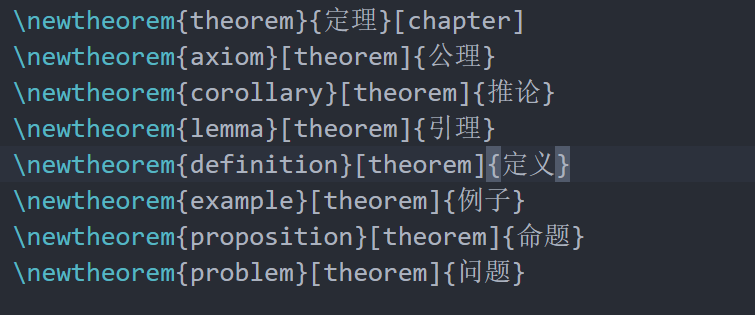
\includegraphics[width=1\textwidth]{manual/figures/定理环境}
  \caption{根据此图做对应修改可插入引理、推论等,具体代码可看latex开头部分环境定义}
  \label{fig_定理环境}
\end{figure}



\section{缩略词输入}

要生成缩略词列表,需要在导言区加入\verb+\makeglossaries+命令,同时在表显示的位置需使用\verb+thesisglossarylist+命令,编译时需要增加makeglossaries main-thesis指令。

% \newacronym[description=基于角度信息的多智能体系统编队控制]{formation}{FMAS}{angle based formation control of multi-agents}

% \gls{formation}使用方法

\section{表格插入}

\begin{table}[h]
  \caption{工作进度安排}
\centering
\setlength{\tabcolsep}{12mm}{
\begin{tabular}{|c|c|c|}
\hline
序号 & 时间                  & 内容      \\ \hline
1  & 20xx.1.8-20xx.1.12  & xxx     \\ \hline
2  & 20xx.3.12-20xx.3.18 & xxx   \\ \hline
\end{tabular}}
\label{gra_process}
\end{table}

\section{算法设计}

\begin{algorithm}[H]
    \KwIn {西瓜集}
    \KwOut{分类结果}
    初始化\;
    \While{迭代未终止}{
        学习\;
        \eIf{西瓜属性}{
            统计\;
            计算\;
        }{
            下一次迭代\;
        }
    }
    \caption{西瓜集分类算法}
\end{algorithm}

\section{glossary}
\appendGlossariesDefinition{
  \newglossaryentry{HDU}{
    name={HDU},
    description={杭州电子科技大学},
    long={Hangzhou Dianzi University},
  }
}
\gls{HDU}

}{}

\chapter{总结与展望}
  \section{总结}
    \subsection{总结1}
    \subsection{总结2}
    \subsection{总结3}
    \subsection{总结4}
  \section{展望}

% 致谢

\acknowledgement
   
当蜘蛛网无情地查封了我的炉台,当灰烬的余烟叹息着贫困的悲哀,我依然固执地铺平失望的灰烬,用美丽的雪花写下:相信未来。

当我的紫葡萄化为深秋的露水,当我的鲜花依偎在别人的情怀,我依然固执地用凝霜的枯藤,在凄凉的大地上写下:相信未来。

我要用手指那涌向天边的排浪,我要用手掌那托住太阳的大海,摇曳着曙光那枝温暖漂亮的笔杆,用孩子的笔体写下:相信未来。

我之所以坚定地相信未来,是我相信未来人们的眼睛——她有拨开历史风尘的睫毛,她有看透岁月篇章的瞳孔。不管人们对于我们腐烂的皮肉,那些迷途的惆怅、失败的苦痛,是寄予感动的热泪、深切的同情,还是给以轻蔑的微笑、辛辣的嘲讽。

我坚信人们对于我们的脊骨,那无数次的探索、迷途、失败和成功,一定会给予热情客观、公正的评定,是的,我焦急地等待着他们的评定。

朋友,坚定地相信未来吧,相信不屈不挠的努力,相信战胜死亡的年青,相信未来,热爱生命。




% 参考文献
\hdubibliography{ref/reference}
%\bibliographystyle{hdu-thesis}
%\bibliography{ref/reference}

% 个人成果
\ifreviewhead
  
\chapter*{作者在读期间发表的学术论文及参加的科研项目}

\subsection*{一、已发表(包括已录用待发表)的论文}

\begin{longtable}{|p{0.6cm}|p{6cm}|p{2.2cm}|p{2cm}|p{2cm}|p{2cm}|}
  \hline
    序号 & 
    发表或投稿刊物/会议名称 & 
    作者(仅注明第几作者)& 
    发表年份 & 
    与学位论文哪一部分(章、节)相关 & 
    被索引收录情况 \\
  \hline
  1 & IEEE Transactions on Instrumentation and Measurement & 第一作者 & 2022 年 & 第四章 & 已索引 \\
  \hline
  2 & Journal of Neuroscience Methods & 第一作者 & 2022 年 & 第二章 & 已索引 \\
  \hline
  3 & Egyptian Informatics Journal & 导师第一, 本人第二 & 2021 年 & 第四章 & 已索引 \\
  \hline
  4 & Journal of Intelligent \& Fuzzy Systems & 第一作者 & 2021 年 & 第二章 & 已索引 \\
  \hline
  5 & IEEE Transactions on Instrumentation and Measurement & 导师第一, 本人第二 & 2022 年 & 第三章 & 已索引 \\
  \hline
\end{longtable}

\subsection*{二、与学位论文内容相关的其它成果(包括专利、著作、获奖项目等)}

\begin{itemize}
    \item[] 专利:已授权三项发明专利,第二/三/三发明人,2021 年 12 月。
    \item[] 著作:参与软件著作一项,第一作者,2022 年 1 月。
    \item[] 获奖项目:获研究生国家奖学金 3 次,第一获奖人,2021 年-2023 年。
\end{itemize}
\else
  \personalAchievements
  张三,男,xxxx年x月生。
目前在杭州电子科技大学自动化学院攻读控制科学与工程博士学位。
当前研究方向包括自主无人系统等。\\

\noindent
\textbf{攻读XX期间的主要成果:}

\begin{enumerate}
  \item  xxxxx. 
  \newblock Stability analysis for a class of switched systems under
    perturbations with applications to consensus[J].
  \newblock IET Control Theory \& Applications, 
    2017, 11(9):1341-1350. (SCI)
  \item xxxx.
    \newblock Consensus of Discrete-time Multi-agent Systems with Decaying Multiplicative Uncertainties[C].
    \newblock Chinese Automation Congress, 2018. (录用)
%%%%%%%%%%%%%%%%%%%%%%%%%%%%%%%%%%%%%%%%%%%%%%%
\end{enumerate}
\fi


% % %%%%%%%%%%%%%%%%%%%%%%%%%%%%%附录%%%%%%%%%%%%%%%%%%%%%%%%%%%%%%%%%%%%
%%%%%\singleappendix(只用一章来可用此命令)
% \singleappendix
% \section{伯努利实验}

% \section{高斯分布}
%%%%%\thesisappendix(多章用此命令)
\thesisappendix

\chapter{大数定理的证明}
  \section{伯努利实验}
  \section{高斯分布}
    \subsection{高斯分布}
\chapter{中心极限定理的证明}
  \section{小节}
%%%%%%%%%%%%%%%%%%%%%%%%%%%%%%%%%%%%%%%%%%%%%%%%%%%%%%%%%%%%%%%%%%%%%


\end{document}
